\documentclass[12pt]{article}

%%%%% Preamble

%% Packages to use

\usepackage{amsmath,amsfonts,amssymb}   %% AMS mathematics macros
\usepackage{graphicx} %% Package to import images.
\usepackage{pagecolor}% http://ctan.org/pkg/{pagecolor}
\usepackage{float}
\usepackage{hyperref}



%% Title Information.
\title{UNIT’s Resources v1.0.0}
\author{Ibai Basabe}
\date{}           %% By default, LaTeX uses the current date

%%%%% The Document

\begin{document}


\pagecolor{white}

\maketitle

\begin{abstract}

UNIT is Crypto’s indexed unit of account. Here we describe UNIT governance resources in detail.

\end{abstract}

\tableofcontents
\newpage



\section{Introduction}

In this document, we describe the distribution of UNIT resources. UNIT governance is the DAO that governs UNIT’s main algorithm and processes to establish an index that can serve as a crypto benchmark and a crypto-native unit of account. For a complete description of UNIT’s main algorithm, see \cite{B1}.

\subsection{Note about the Usage of this Document}

This document has been prepared for information purposes only. It is not soliciting any action from the reader. The contents of this document are subject to change.


\section{Resource Economics}

\subsection{UNIT's Resources}

UNIT’s governance token, UN, is the controlling voting unit governing UNIT’s algorithm. The maximum amount to ever enter circulation is $2^{33}$ UN tokens.





\newpage

\subsection{Allocation}

UN is allocated as shown in Figure \ref{fig:allocation}. 

\begin{figure}[h!]
\centering
  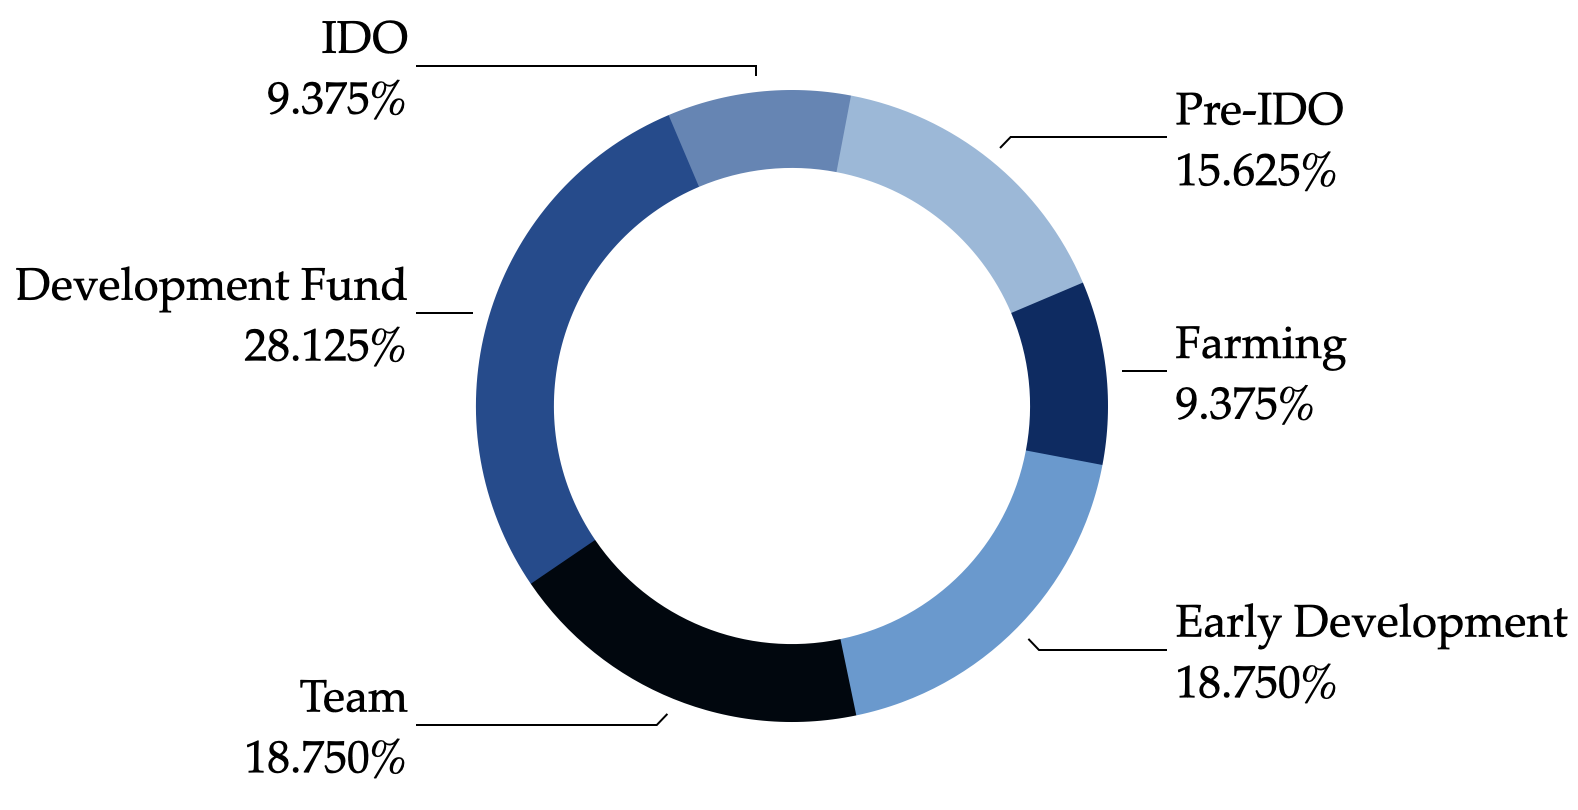
\includegraphics[width=5in]{images/UN_Allocation.png}
  \caption{Total allocation.}
  \label{fig:allocation}
\end{figure}



\subsection{Vesting}

An amount of the initial UN will be vested for the times defined in Figure \ref{fig:allocation_timeline}. Team, Early Development, Pre-IDO, and Development Fund will have vesting schedules. For an allocation schedule with inflation rates see Figure \ref{fig:allocation_timeline}.


\begin{figure}[H]
\centering
  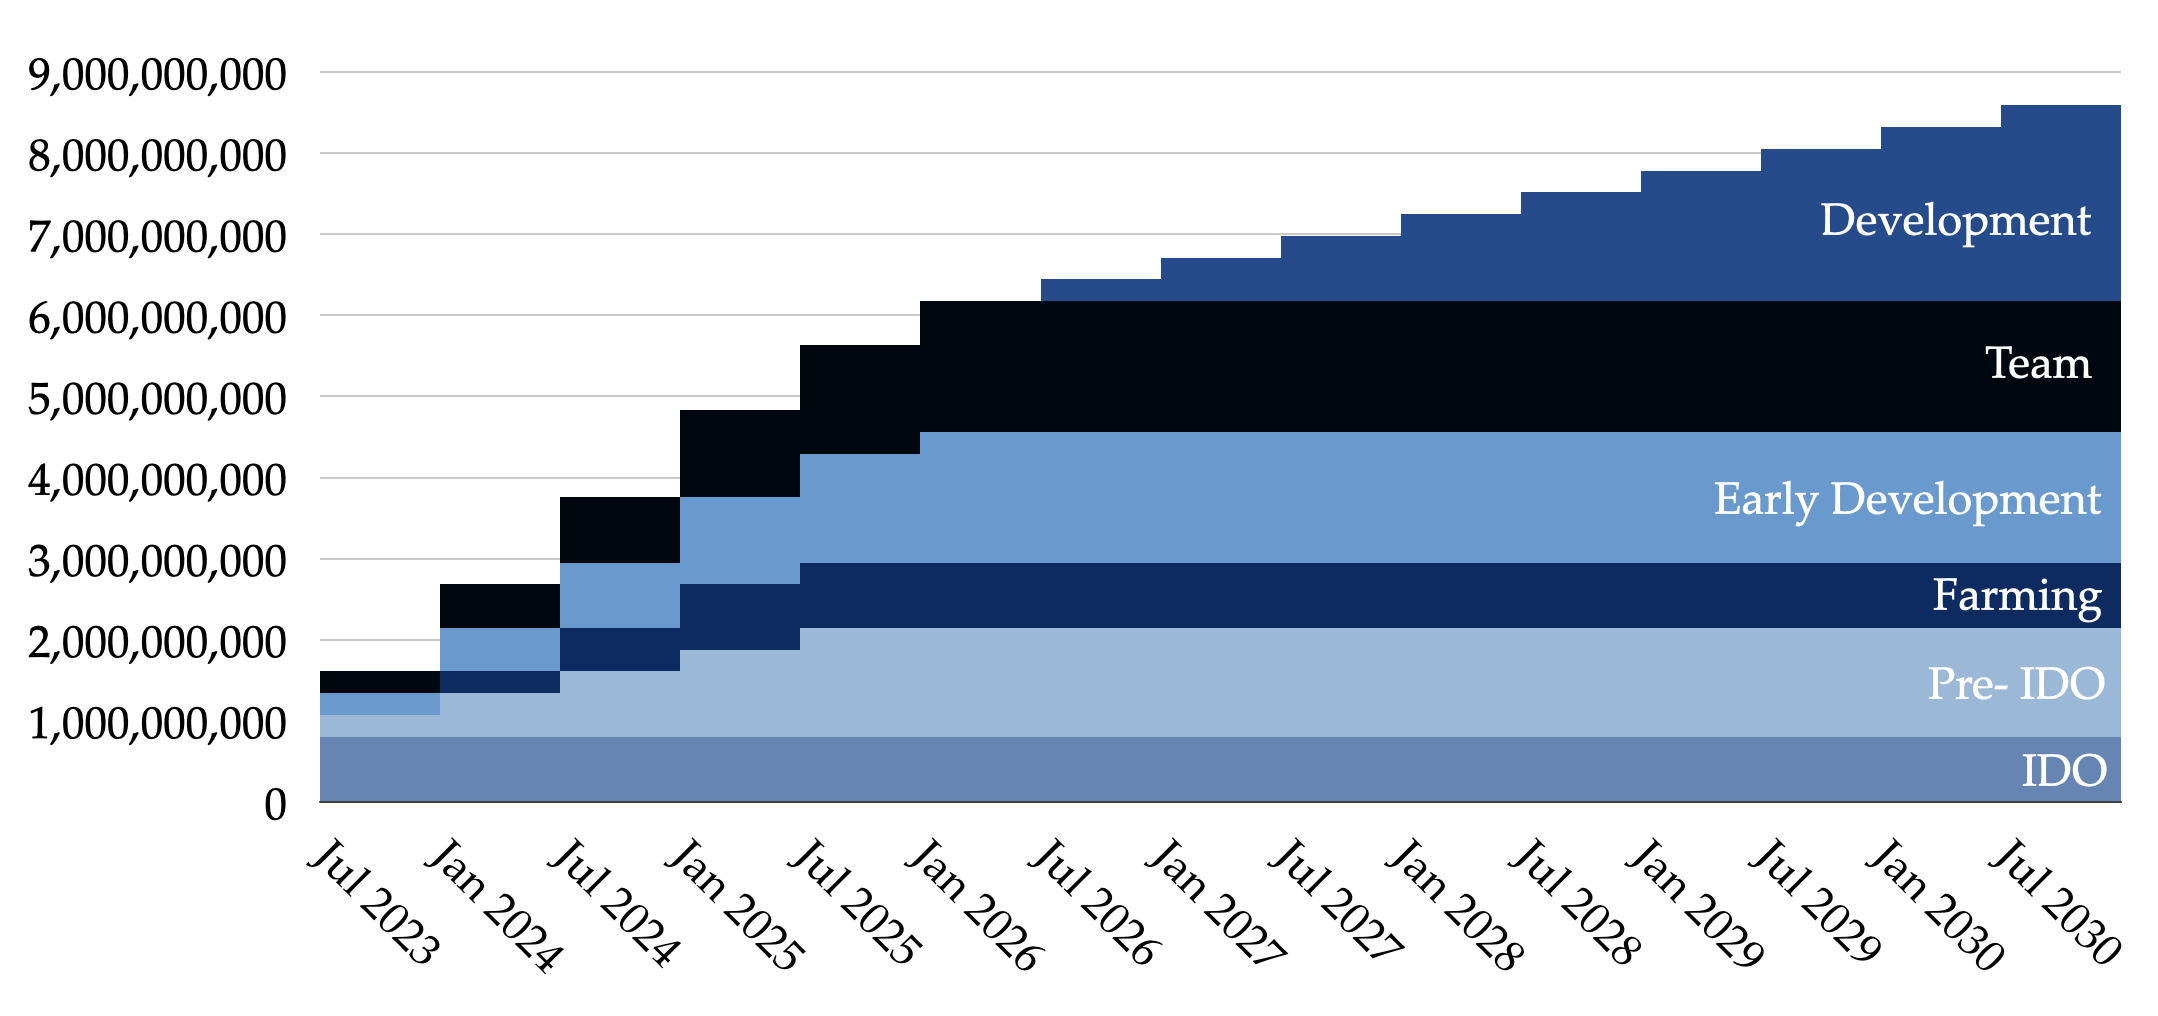
\includegraphics[width=5in]{images/UN_Allocation_Timeline.png}
  \caption{Allocation with vesting details}
  \label{fig:allocation_timeline}
\end{figure}







\section{Development Links}

UNIT’s ideas started in 2018; however, it was not as necessary in the crypto space then as it is today. Therefore, the project began testing the hypothesis of an indexed unit of account in 2021. It is now running strong towards executing the plan.

We first launched UNIT’s algorithm online on May 5, 2021. Currently. Follow our development at \href{http://www.unitindex.org}{unitindex.org}.

\begin{thebibliography}{[BLSWZ9]}
\bibliographystyle{amsalpha}

\bibitem[B1]{B1} Basabe, I.: The Unit: Establishing a Crypto-Native Unit of Account. \emph{https://github.com/toknowwhy/the-unit-paper} (2020).


\bibitem[B2]{B2} Basabe, I.: 2ØY's (To Know Why) Values. \emph{https://github.com/toknowwhy/20y-values-paper} (2019).



\end{thebibliography}



\end{document}
